\documentclass{ucbthesis}

\usepackage{amsfonts}
\usepackage{amssymb}
\usepackage{biblatex}
\usepackage{color}
\usepackage{graphicx}
\usepackage{hyperref}
\usepackage{listings}
\usepackage{multirow}
\usepackage{subcaption}
\usepackage{times}
\usepackage[T1]{fontenc}

\lstset{
  showspaces=false,
  showtabs=false,
  breaklines=true,
  showstringspaces=false,
  breakatwhitespace=true,
  escapeinside={(*@}{@*)},
  basicstyle=\small\ttfamily,
  columns=fullflexible,
  morekeywords={maybe_downsample, maybe_skip}
}

%% \def\dsp{\def\baselinestretch{2.0}\large\normalsize}
%% \dsp

\bibliography{thesis}

\begin{document}

\title{ A Proposal for Adaptive Wide-area Streaming Analytics }

\author{ Ben Zhang }
\degreesemester{XX}
\degreeyear{XXXX}
\degree{Doctor of Philosophy}
\chair{Professor John Wawrzynek}
\othermembers{Professor Edward A. Lee \\
  Professor Sylvia Ratnasamy \\
  Professor John Chuang}
\field{Computer Science}
\campus{Berkeley}
\numberofmembers{3}

\maketitle
%% \approvalpage
%% \copyrightpage

\newcommand{\sysname}{AdaptiveStream}

\definecolor{todo}{rgb}{1, 0, 0}
\definecolor{ben}{rgb}{0.5, 0.5, 0.0}
\definecolor{xin}{rgb}{0.0, 0.5, 0.5}

\newtoggle{anonymous}
\toggletrue{anonymous}
%\togglefalse{anonymous}

\newtoggle{comments}
\toggletrue{comments}
% \togglefalse{comments}

\iftoggle{comments} {
  % show comments with the corresponding color
  \newcommand {\ben}[1]{{\color{ben}\bf{BZ: #1}\normalfont}}

  \newcommand {\todo}[1]{{\color{todo}TODO: #1}\normalfont}
}{
  % do not show comments
  \newcommand {\ben}[1]{}

  \newcommand {\todo}[1]{}
}

\newcommand{\squishlist}{
  \begin{list}{$\bullet$}
    { \setlength{\itemsep}{0pt}
      \setlength{\parsep}{3pt}
      \setlength{\topsep}{3pt}
      \setlength{\partopsep}{0pt}
      \setlength{\leftmargin}{1.5em}
      \setlength{\labelwidth}{1em}
      \setlength{\labelsep}{0.5em} } }
  \newcommand{\squishend}{
  \end{list}  }

\newcommand{\boldhead}[1]{\vspace{0.5em}\noindent\textbf{#1}}

\newcommand{\para}[1]{\vspace{0.6em}\noindent\textbf{#1}}
\newcommand{\paraf}[1]{\vspace{0.1em}\noindent\textbf{#1}}

\newcommand{\specialcell}[2][c]{%
  \begin{tabular}[#1]{@{}c@{}}#2\end{tabular}}

\renewcommand*\chapterautorefname{Chapter}
\renewcommand*\sectionautorefname{Section}
\renewcommand*\subsectionautorefname{Section}
\renewcommand*{\equationautorefname}{Eq.}
\renewcommand*{\figureautorefname}{Fig.}

%%% Local Variables:
%%% mode: latex
%%% TeX-master: "sigcomm2017"
%%% End:

%%% Local Variables:
%%% mode: latex
%%% TeX-master: "thesis"
%%% End:


\begin{abstract}

  The swarm refers to the vast collection of networked sensors and actuators
  installed in our connected world. Many swarm applications generate, transport,
  distill, and process large streams of data across the wide area in real
  time. The increasing volume of data generated at the edge challenges the
  existing approaches of directly connecting devices to the cloud.

  This thesis begins with an overview of emerging swarm and the architecture
  design trends for swarm applications. The swarm faces challenges from the
  scarce and variable WAN bandwidth and the heterogeneous compute environment
  (from low-power microcontrollers to powerful compute units). When network
  resources or compute resources are insufficient, non-adaptive applications
  will suffer from increased latency or degraded accuracy. Existing approaches
  that support adaptation either require extensive developer effort to write
  manual policies or are limited to application-specific solutions.

  This thesis proposes a systematic and quantitative approach to build adaptive
  swarm applications. The solution has three stages: (1) a set of programming
  abstractions that allow developers to express adaptation options; (2) an
  automatic profiling tool that learns an accurate profile to characterize
  resource demands and application performance; (3) a runtime system responsive
  to environment changes, maximizing application performance guided by the
  learned profile.

  We evaluate our methodology with adaptations to network resources and compute
  resources. For network resources, we present a complete design and
  implementation of the framework \awstream{} and several swarm applications:
  pedestrian detection, augmented reality, and monitoring log analysis. Our
  experiments show that all applications can achieve sub-second latency with
  nominal accuracy drops. For compute resources, we focus on improving the
  profiling efficiency---using Bayesian Optimization to address the large
  parameter space and profile transfer to address device heterogeneity.

\end{abstract}

%%% Local Variables:
%%% mode: latex
%%% TeX-master: "thesis"
%%% End:


\pagestyle{headings}
\section{Introduction}
\label{sec:introduction}

An increasing number of swarm applications rely on heavy computation tasks,
notably machine learning (ML) applications. For example, Microsoft
SeeingAI~\cite{seeingai} is a talking camera for the blind and low vision
community that describes nearby people, text, objects, etc. Wearable cognitive
assistant~\cite{ha2014towards} uses wearable devices, such as Google Glass, for
deep cognitive assistance, e.g., offering hints for social interaction via
real-time scene analysis.

While there is a staggering collection of research focusing on model
\textit{training} for these tasks, for swarm applications, they perform the
\textit{inference} step of machine learning: it uses a trained model to make a
prediction given an input, such as visual~\cite{googlelens, ha2014towards,
  seeingai}, audio~\cite{alexa, applesiri, cortana}, and sensory
information~\cite{laput2017synthetic, lu2010jigsaw}. Inference has received
relatively little attention, especially on edge and end devices.

One important challenge for inference is to bound the response time, which
affects user experience significantly in these human-in-the-loop
systems. Previous usability studies~\cite{nielsen1994usability,
  schneiderman1998designing} have measured the effect of different end-to-end
response times:

\begin{itemize}[noitemsep, topsep=0pt]
\item 100 ms gives the feeling of instantaneous response.
\item 1 second keeps the user's flow of thought but users can sense the delay.
\item A few seconds' delay creates an unpleasant user experience.
\end{itemize}

Achieving bounded response times (BRT) on swarm devices has remained
challenging. Swarm devices are extremely heterogeneous and many are resource
constrained (see \autoref{tab:embedded}). Heavy computations can be simply
beyond the capabilities of cheap end devices. For example, state-of-the-art
object detection algorithm easily takes several seconds on modern
smartphones~\cite{chen2015glimpse}.

To compensate resource-constrained devices, prior work explores
offloading~\cite{chun2011clonecloud,cuervo2010maui} to the cloud or the edge
that hosts machine learning models and performs heavy computation. Despite their
powerful computing capability and more available resources, e.g., special
hardware like GPU and TPU~\cite{jouppi2017datacenter}, these machines suffer
from increased network latency and service overload (\autoref{fig:edge}). As a
result, they are often unable to meet response time goals consistently.

Another technique for low latency is to use redundant requests. By initiating
multiple requests across a diverse set of resources and using the first result
that completes, redundancy is effective to address the variability in network
delays~\cite{gordon2015accelerating, vulimiri2013low} and slow servers (known as
straggler mitigation in the cloud~\cite{dean2013tail,
  ananthanarayanan2013effective}). However, existing works treat these resources
equally and execute the same task on each platform, a poor match for the
heterogeneous swarm space.

We make the observation that for a particular task, there are many options:
different algorithms or tunable parameters for the same algorithm. These options
result in different processing times and application accuracy. If we can adapt
the computation by choosing an option that matches the capability of the device
or satisfy the deadline requirement, we can achieve bounded response times.

The idea of adapting to machines is illustrated in \autoref{fig:dr}. It builds
on top of redundancy but addresses, or rather leverages, the heterogeneity of
swarm devices.  On-device processing can use a simple algorithm if the device is
resource constrained. The device also sends redundant requests to other servers,
e.g., the edge and/or the cloud. Each request contains a service-level objective
(SLO) that describes the deadline and accuracy demand. Upon receiving the
request, the server would admit or reject the request based on the network
delays and its workload. Because of the redundancy, rejection is fine. This is
different from traditional web serving where the server is the single point of
source. At last, the device would use the first response that completes.

\begin{figure}
  \centering
  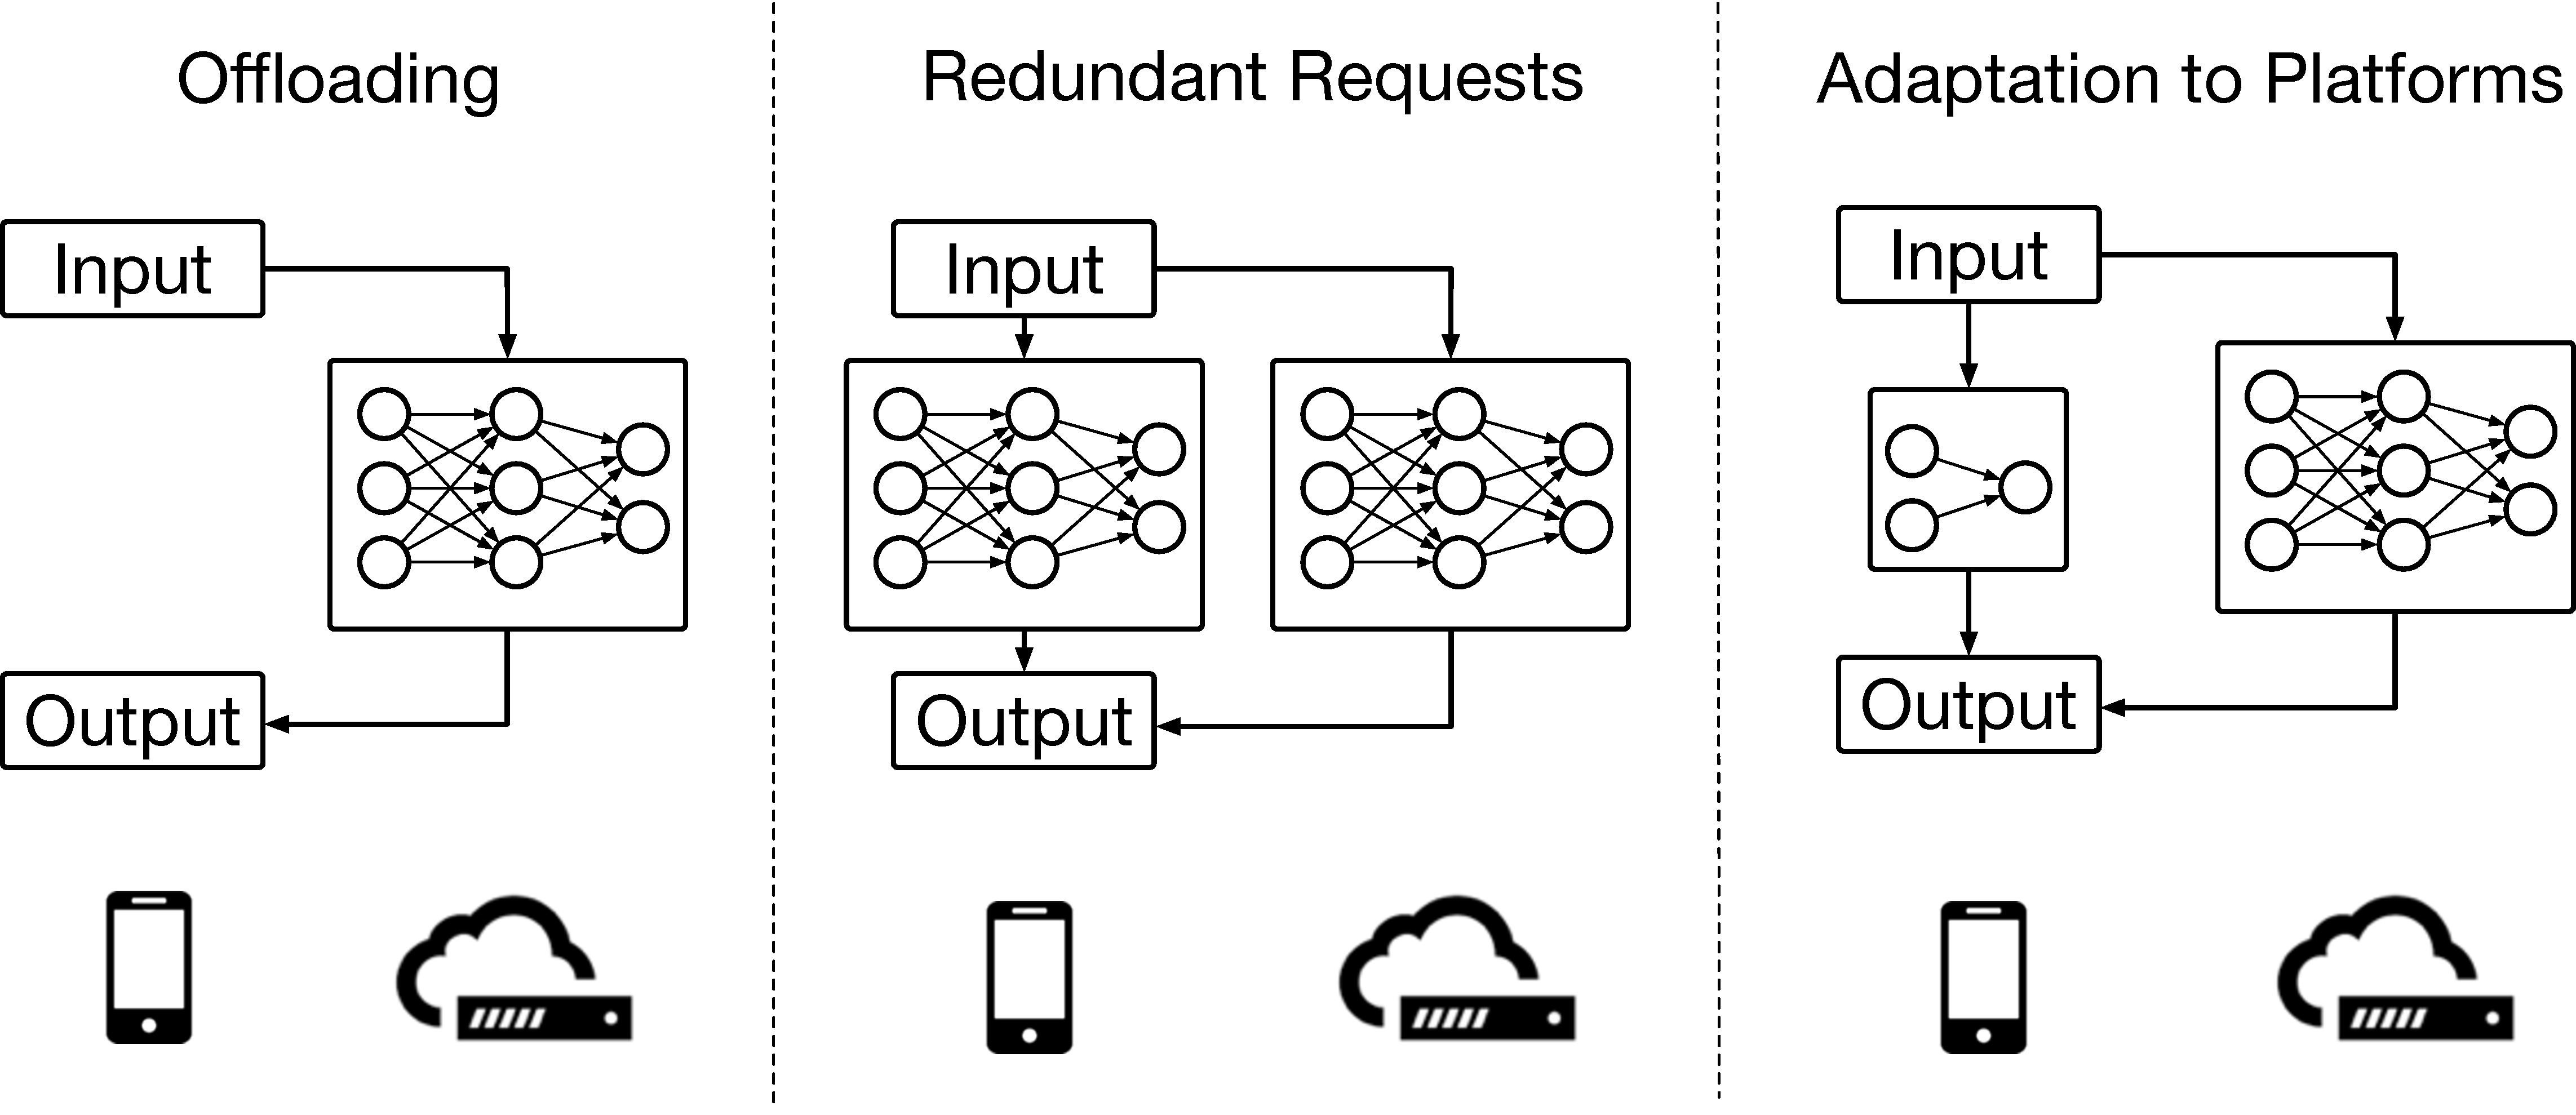
\includegraphics[width=0.8\columnwidth]{figures/dr.pdf}
  \caption{Illustration of offloading, redundant requests and compute
    adaptation.}
  \label{fig:dr}
\end{figure}

The key to enable adaptation lies in building an accurate performance model that
characterized the processing times and accuracy trade-off for a particular
task. We take a data-driven approach by measuring processing times and accuracy
for a given set of training data. We call this process profiling and the
resulting performance model is the profile.

Efficient profiling is challenging given the large space formed by the
combination of algorithms, parameters, and machines. We need to profile each
algorithms individually. For a single algorithm, it may have a huge parameter
space. For example, cascading classifiers in computer vision tasks have
configurable convolution window size, scale factor, and minimum neighbor for non
maximum suppression. Exhaustive profiling this space is prohibitively expensive
(see \autoref{fig:vj-tradeoff}). Because processing times depend on the devices,
the profile is different across devices. It is infeasible to profile all
hardware platforms because of the staggering number of devices and their
availability at development time.

In this chapter, we discuss techniques to efficiently build the performance
model for compute adaptation in an automated, data-driven way. We first describe
our programming language abstractions that allow developers to specify different
algorithms and their parameters. We then build the profiler. \todo{more.}

This chapter make the following contributions regarding performance modeling:

\begin{enumerate}[noitemsep, topsep=0pt]
\item To address the large parameter space, we use Bayesian Optimization (BO)
  for profiling to learn the Pareto-optimal set of parameters. We show that BO
  outperforms baseline approaches, including random search and coordinate
  search.
\item We propose to transfer profiles across devices without running the
  profiling again. New machines only need to sample a fraction of the
  Pareto-optimal set and measure the processing times only.
\end{enumerate}

%%% Local Variables:
%%% mode: latex
%%% TeX-master: "../compute"
%%% End:

\chapter{\sysname{} Design}
\label{sec:system-design}

In this chapter, I present the design of \sysname{}. The primary goal of
\sysname{} is to empower applications with the ability to adapt its
communication while maximizing the utility.

\section{Challenges}
\label{sec:challenges}

\noindent There are four challenges in realizing \sysname{}.

\para{C1: Diverse application and data:} As discussed in~\autoref{sec:bat}, the
best adaptation scheme is often application- and context-specific
optimizations. It becomes important to separate individual application logic
from specific degradation strategy as well as the concrete mechanisms.

\para{C2: No analytical solutions:} Unlike SQL queries whose demand and accuracy
can typically be estimated using analytical models~\cite{cormode2012synopses},
many of our streaming applications are dealing with unstructure data using
either use blackbox operations (such as H.264 encoding) or non-linear operators
(such as thresholding). The effect of these degradations is not immediately
available.

\para{C3: Multi-dimensional exploration:} Real-world applications typically have
more than one tunable parameters; leading to a combinatorial space for
exploration. In addition, these parameters are not necessarily orthognal.  The
optimal degradation strategies may only be achievable when more than one
degradation is in effect.

\para{C4: Runtime adaptation at application layer:} Although recent work on
resource reservation makes it possible to guarantee quality of service with new
IP or MAC layer protocols in LAN (e.g. TSN~\cite{johas2013heterogeneous}), we
target at WAN analytics where most of the infrastructure is owned by others and
shared among many users. An application-layer solution is in favor to those that
require special hardware or software upgrade.

\section{System Architecture}
\label{sec:architecture}

\begin{figure*}
  \centering
  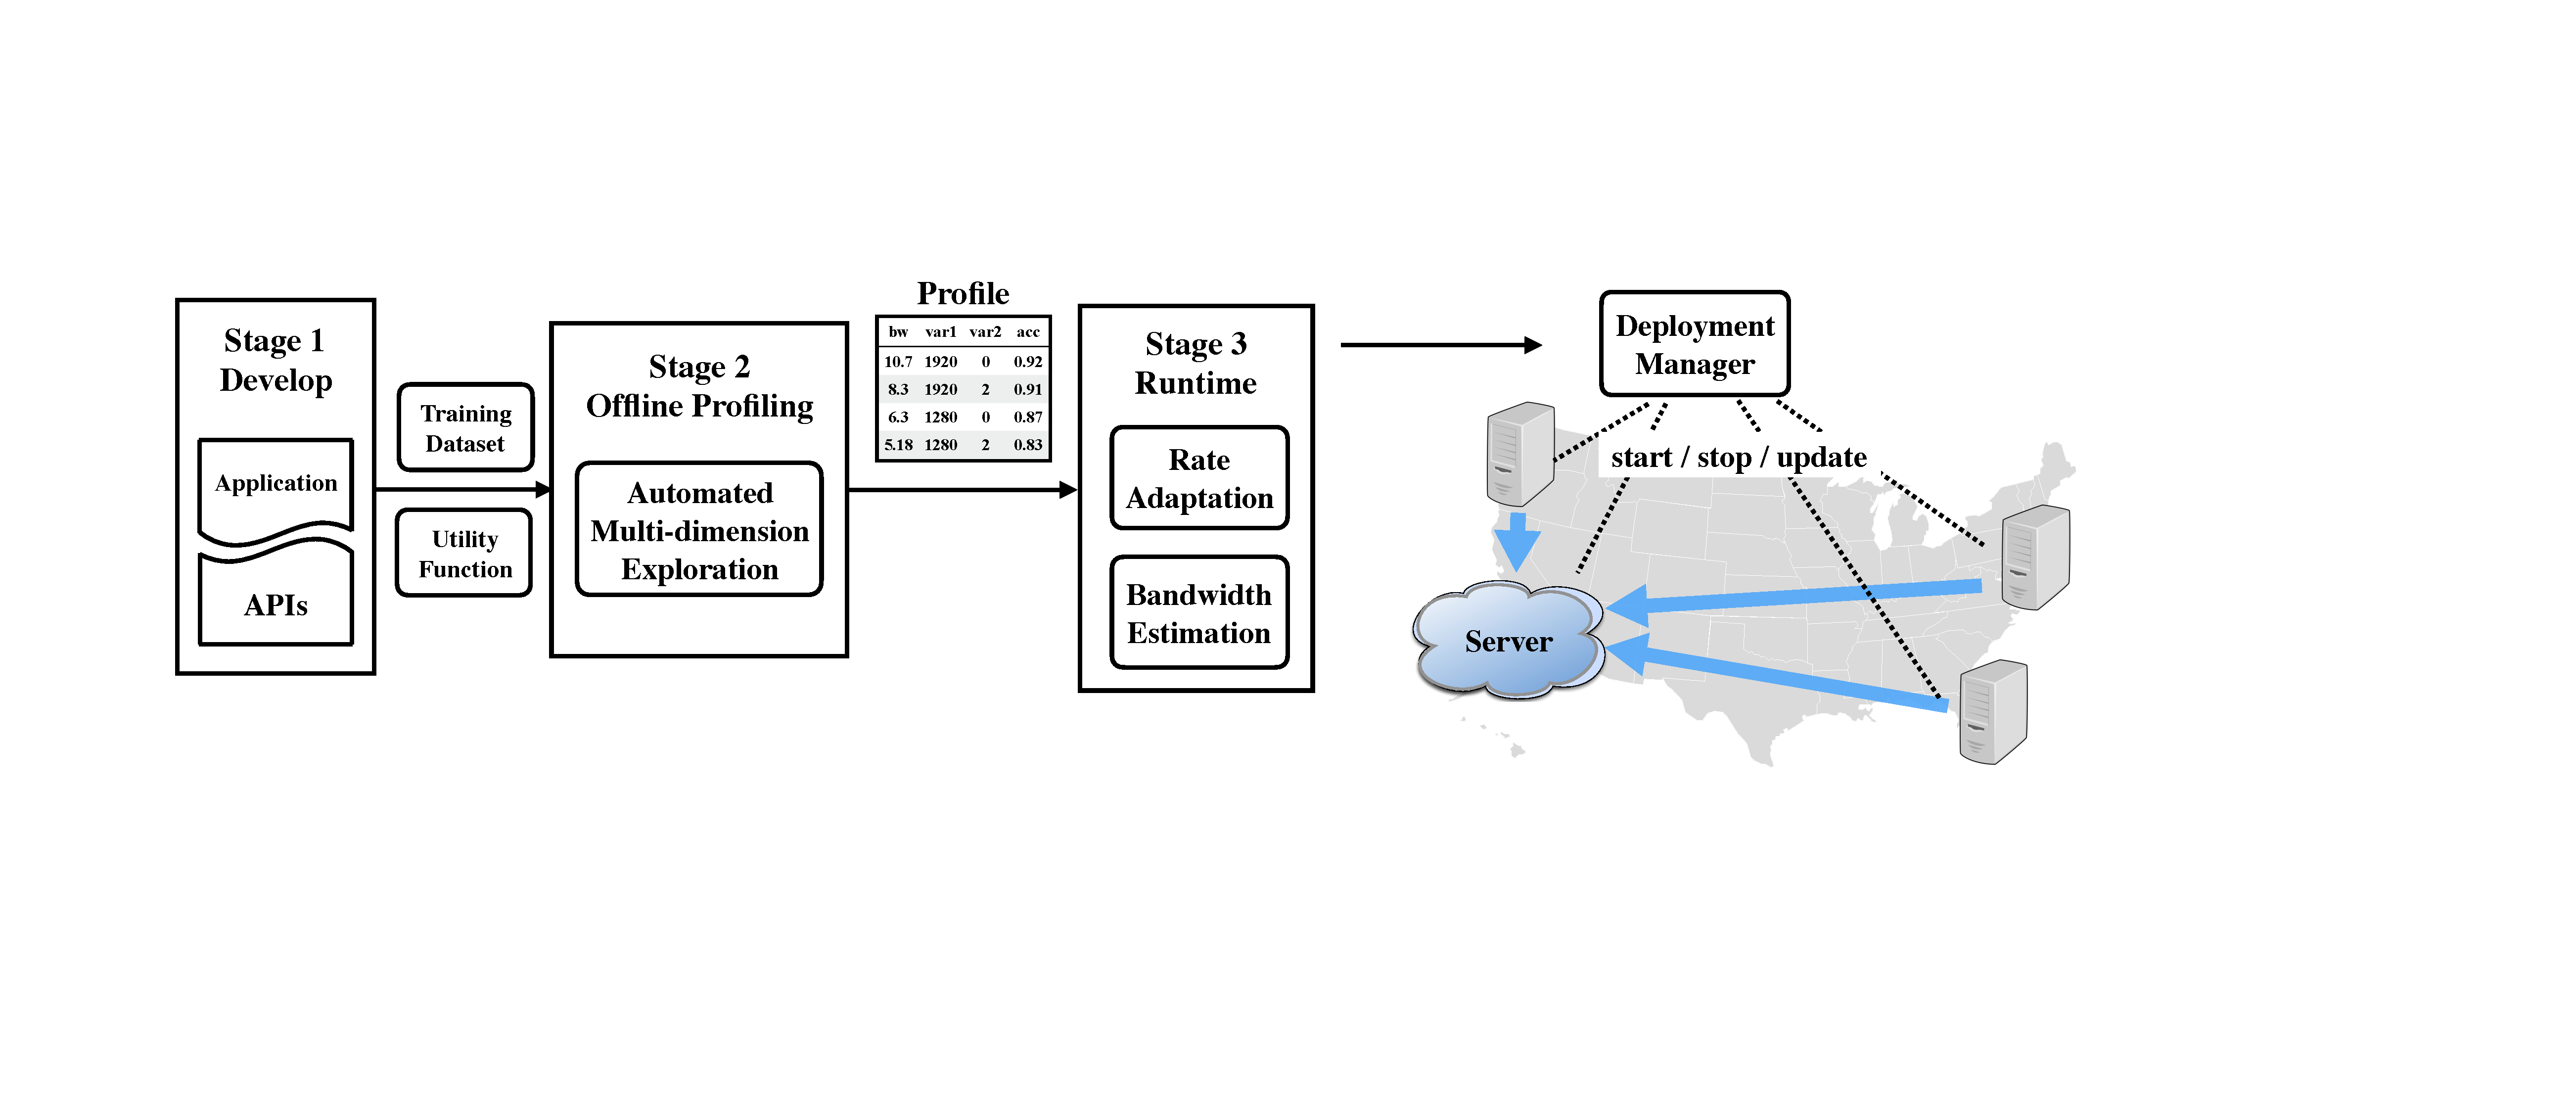
\includegraphics[width=\linewidth]{figures/arch.pdf}
  \caption{The three-stage architecture of \sysname{}.}
  \label{fig:overview}
\end{figure*}

To address the aforementioned challenges, \sysname{}'s solution is split into
three parts (\autoref{fig:overview} illustrates them).

\para{Programming abstraction~(\autoref{sec:prog-abs}):} Applications are
modelled as a directed acyclic graph (DAG) of computations. In addition to the
normal operators from existing systems, I propose a novel set of \texttt{maybe}
operators to express the specification of degradations. The proposed APIs do not
require developers to be exact on the quantity, making effort to integrate with
existing applications minimal.

\para{Automatic multi-dimensional profiling~(\autoref{sec:profiling}):} The
system automatically explores the parameter space to learn a Pareto-optimal
degradation strategy in a application-specific manner. This process frees
application developers from a tedious and repetitive process.

\para{Runtime Adaptation~(\autoref{sec:adaptation}):} Finally the streaming
application is deployed with a wide-area orchestration manager. At runtime,
\sysname{} provides all the necessary modules that act as the control plane and
adapt the application execution. At a high level, it performs bandwidth
estimation, congestion monitoring and adaptation. It uses the profile learned
from the second stage to guide the level of degradation.

\section{Programming Abstraction}
\label{sec:prog-abs}

Applications in \sysname{} are composed by connecting a set of operators to form
a dataflow graph. The system provides a basic set of APIs such as \texttt{map},
\texttt{filter}, \texttt{window} (\autoref{tab:operators}). The normal operators
are similar to existing stream processing systems; the core contribution of this
thesis is the set of \texttt{maybe} APIs that allows the specification of
degradation operations for bandwidth-accuracy trade-off.

\begin{table*}
  \small
  \centering
  \begin{tabular}{ c r l }
    \toprule
    \multirow{7}{*}{\begin{tabular}{@{}c@{}}Normal \\ Operators\end{tabular}}
    & \textit{map}(f: I $\Rightarrow$ O) & Stream<I> $\Rightarrow$ Stream<O> \\
    & \textit{filter}(f: I $\Rightarrow$ bool) & Stream<I> $\Rightarrow$
                                                 Stream<I> \\
    & \textit{skip}(i: Int) & Stream<I> $\Rightarrow$ Stream<I> \\
    & \textit{sliding\_window}(count: Int, f: Vec<I> $\Rightarrow$ O) & Stream<I> $\Rightarrow$
                                                                            Stream<O> \\
    & \textit{tumbling\_window}(count: Int, f: Vec<I> $\Rightarrow$ O) & Stream<I> $\Rightarrow$
                                                                             Stream<O> \\
    & \textit{timed\_window}(time: Duration, f: Vec<I> $\Rightarrow$ O) & Stream<I> $\Rightarrow$
                                                                          Stream<O> \\
    & ... & ... \\
    \midrule
    \multirow{4}{*}{\begin{tabular}{@{}c@{}}Degradation \\ Operators\end{tabular}}
    & \textit{maybe}(knobs: Vec<T>, f: (T, I) $\Rightarrow$ I) & Stream<I> $\Rightarrow$
                                                                 Stream<I> \\
    & \textit{maybe\_skip}(knobs: Vec<T>) & Stream<I> $\Rightarrow$ Stream<I> \\
    & \textit{maybe\_downsample}(knobs: Vec<(Int, Int)>) & Stream<Image> $\Rightarrow$ Stream<Image> \\
    & ... & ... \\
    \bottomrule
  \end{tabular}
  \caption{A comparison between normal stream processing operators and our
    degradation operators. Vec<T> represents a list of elements of type
    T. Notice the type constrain on the second argument passed to
    \texttt{maybe}.}
  \label{tab:operators}
\end{table*}

\subsection{Degradation Operators}
\label{sec:prog-abs}

To design the degradation operator, let's first consider a strawman solution:
manual policies for degradation. JetStream~\cite{rabkin2014aggregation} offers
an example: ``if bandwidth is insufficient, switch to sending images at 75\%
fidelity, then 50\% if there still isn't enough bandwidth. Beyond that point,
reduce the frame rate, but keep the images at 50\% fidelity.'' This manual
policy specification has the following issues:

\para{Lack of precision:} These policies are often developer heuristics and
rarely backed up by measurements. First, there is no direct association of the
application accuracy with the 75\% fidelity configuration. Besides, the effect
of each rule on the data size is not trivially available.  While it seems
intuitive that the level of degradation will change the data size, the precise
effect is not always straightforward. For example, one might think that reducing
the frame rate by 50\% will half the data rate. When video encoding is employed,
the inter-frame difference will increased (P-frame size) when the frame rate is
reduced. This leads to a larger data size for each frame. \autoref{fig:h264}
illustrates this complex relationship with an example of H.264 encoding under
four different frame rates.

\para{Not scalable:} The strawman solution quickly leads to too many policies
when multiple degradation operations are involved or a fine-grained control is
desired. This manual process becomes tedious and error-prone. When too few rules
are provided, the application may oscillate between two rules: one that's too
aggressive (always faces insufficient bandwidth) and one that's too conservative
(a suboptimal strategy).

\begin{figure}
  \centering
  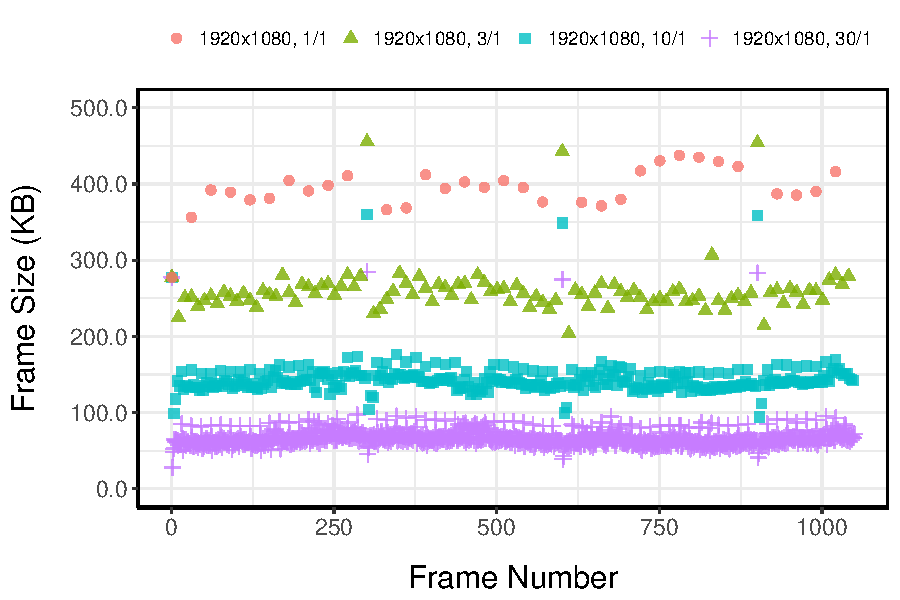
\includegraphics[width=\columnwidth]{figures/h264.pdf}
  \caption{H.264 requires more information per frame when the frame rate is
    reduced. All measurements are for videos with 1920x1080 resolution and the
    same H.264 configurations. 1/1, 3/1, 10/1 and 30/1 in the legend mean that
    the frame rates are 1 FPS, 3 FPS, 10 FPS and 30 FPS.}
  \label{fig:h264}
\end{figure}

\vspace{0.5em}

I argue that when using the above strawman solution, developers are forced to
manually study and measure the effect of individual degradation policy,
prohibiting its wide adoption in practice.

On the other extreme of the design spectrum lies a completely developer-free
solution. It is not practical, either. While static analysis has been shown to
optimize application execution adaptively in a mobile-cloud
context~\cite{chun2011clonecloud}, it only concerns with computation placement
(on the mobile or in the cloud) rather than tuning application parameters.  For
our dataflow programming model, static analysis is prone to false positives:
exploring wrong or unnecessary parameters. For example, when the application is
configured to generates statistics with a \texttt{timed\_window} operation,
static analysis may falsely detect the duration parameter and alter the behavior
of the application in an unexpected way. Also, as we will illustrate
in~\autoref{sec:profiling}, with each introduced parameter, the profiling time
increases drastically as all parameters pose a combinatorial space. The
explosion of search space prohibits explorations of unnecessary parameters.

\sysname{} takes a middle ground between these two extremes: developers use a
novel \texttt{maybe} API to annotate degradation operations without being exact
on the values. Think of these APIs as hints from developers: this operation,
when in use, will likely reduce the data size and affect the data fidelity;
however the exact quantity is not clear.

The basic form of \texttt{maybe} operator takes two arguments: a knob and a
degradation function (see \autoref{tab:operators}). The knob indicates different
degradation levels; the function performs the actual degradation operation with
a configurable level. There is one restriction on the type signature of the
function argument: $f(T, I) \Rightarrow I$. That is, the degradation function
should not alter the type of the stream. While this seems a strong restriction,
when combined with the \texttt{map} operator, the API set is still expressive
enough. I describe the implementation and usage of the APIs
in~\autoref{sec:implementation}.

Based on the \texttt{maybe} primitive, one can implement wrappers for common
degradation operations. For example, \texttt{maybe\_skip} will optionally
subsample a stream; \texttt{maybe\_downsample} can adjust the image resolution
to a configured target. Using the \texttt{maybe} API, the example mentioned
earlier can now be implemented as follows:

\begin{lstlisting}
   let app = Camera::new((1920, 1080, 30))
      .maybe_downsample(vec![(1600, 900), (1280, 720)])
      .maybe_skip(vec![2, 5])
      .map(|frame| frame.show())
      .compose();
\end{lstlisting}

This snippet first instantiates a \texttt{Camera} source, which has the type
\texttt{Stream<Image>}. It's configured to produce images with 1920x1080
resolution and 30 FPS. Two degradation operations are chained after the source:
one that downsamples the resolution to either 1600x900 or 1280x720; the other
skips frames with a parameter of 2 or 5, resulting in $30 / (2+1) = 10$ FPS or
$30/(5+1) = 5$ FPS. After the degradation, images are shown on the display; in
practice, further processing operators can be chained after the degradation.

While the API itself has simplified the specification of degradation, the exact
amount has to be known for precise rate adjustment at runtime. We then turn to
the second stage of our system that performs the automatic profiling.

\section{Multi-dimensional Profiling}
\label{sec:profiling}

The goal of this profiling stage is to explore the bandwidth-accuracy trade-off
and learn a Pareto-optimal \textit{profile} for a specific application and its
target scenario. The profile consists a set of rules that determines how each
degradation operations will configured; each rule is a \textit{(bandwidth,
  configuration)} tuple.

Before we discuss properties of profile, we define the terms and notations
(\autoref{tab:notations}). Each \texttt{maybe} operator within an application
corresponds to a knob $k$. Suppose the application has $n$ knobs, their
combination forms a configuration $c = [k_{1}, k_{2}, ... k_{n}]$. The set of
all configurations $\mathbb{C}$ is the space that the profiling system need to
explore.

There are two mappings that we are interested: a mapping from a particular
configuration to its bandwidth requirement $B(c)$ and the accuracy measure
$A(c)$. The Pareto-optimal set $\mathbb{P}$ can then be defined
(\autoref{eq:pareto}): for all $c \in \mathbb{P}$, there is no alternative
configuration $c'$ that requires less bandwidth while giving a higher accuracy.

{\small
\begin{equation}
  \mathbb{P} = \{ c \in \mathbb{C} : \{ c' \in \mathbb{C}: B(c') < B(c),
  A(c') > A(c) \} = \varnothing\}
  \label{eq:pareto}
\end{equation}
}%

\begin{table}
  \centering
  \begin{tabular}{r l}
    \toprule
    \textbf{Symbol} & \textbf{Description} \\
    \midrule
    $n$ & number of degradation operations \\
    $k_i$ & the \textit{i}-th degradation knob \\
    $c = [k_{1}, k_{2}, ... k_{n}]$ & one specific configuration \\
    $\mathbb{C}$ & the set of all configurations \\
    \midrule
    $B(c)$ & bandwidth requirement for $c$ \\
    $A(c)$ & accuracy measure for $c$ \\
    $\mathbb{P}$ & Pareto-optimal set \\
    \bottomrule
  \end{tabular}
  \caption{Notations used in profiling.}
  \label{tab:notations}
\end{table}

Since there is often no close-form relation for $B(c)$ and $A(c)$, for arbitrary
degradation operations, \sysname{} takes a data-driven approach. With a
representative dataset and an application-specific utility function, the system
evaluates each configuration for the bandwidth demand and the application
utility. The utility could either be measured against the groundtruth; or in the
case when labelled dataset is not available, the system uses the reference
results when all degradations are turned off.

\begin{figure}
  \centering
  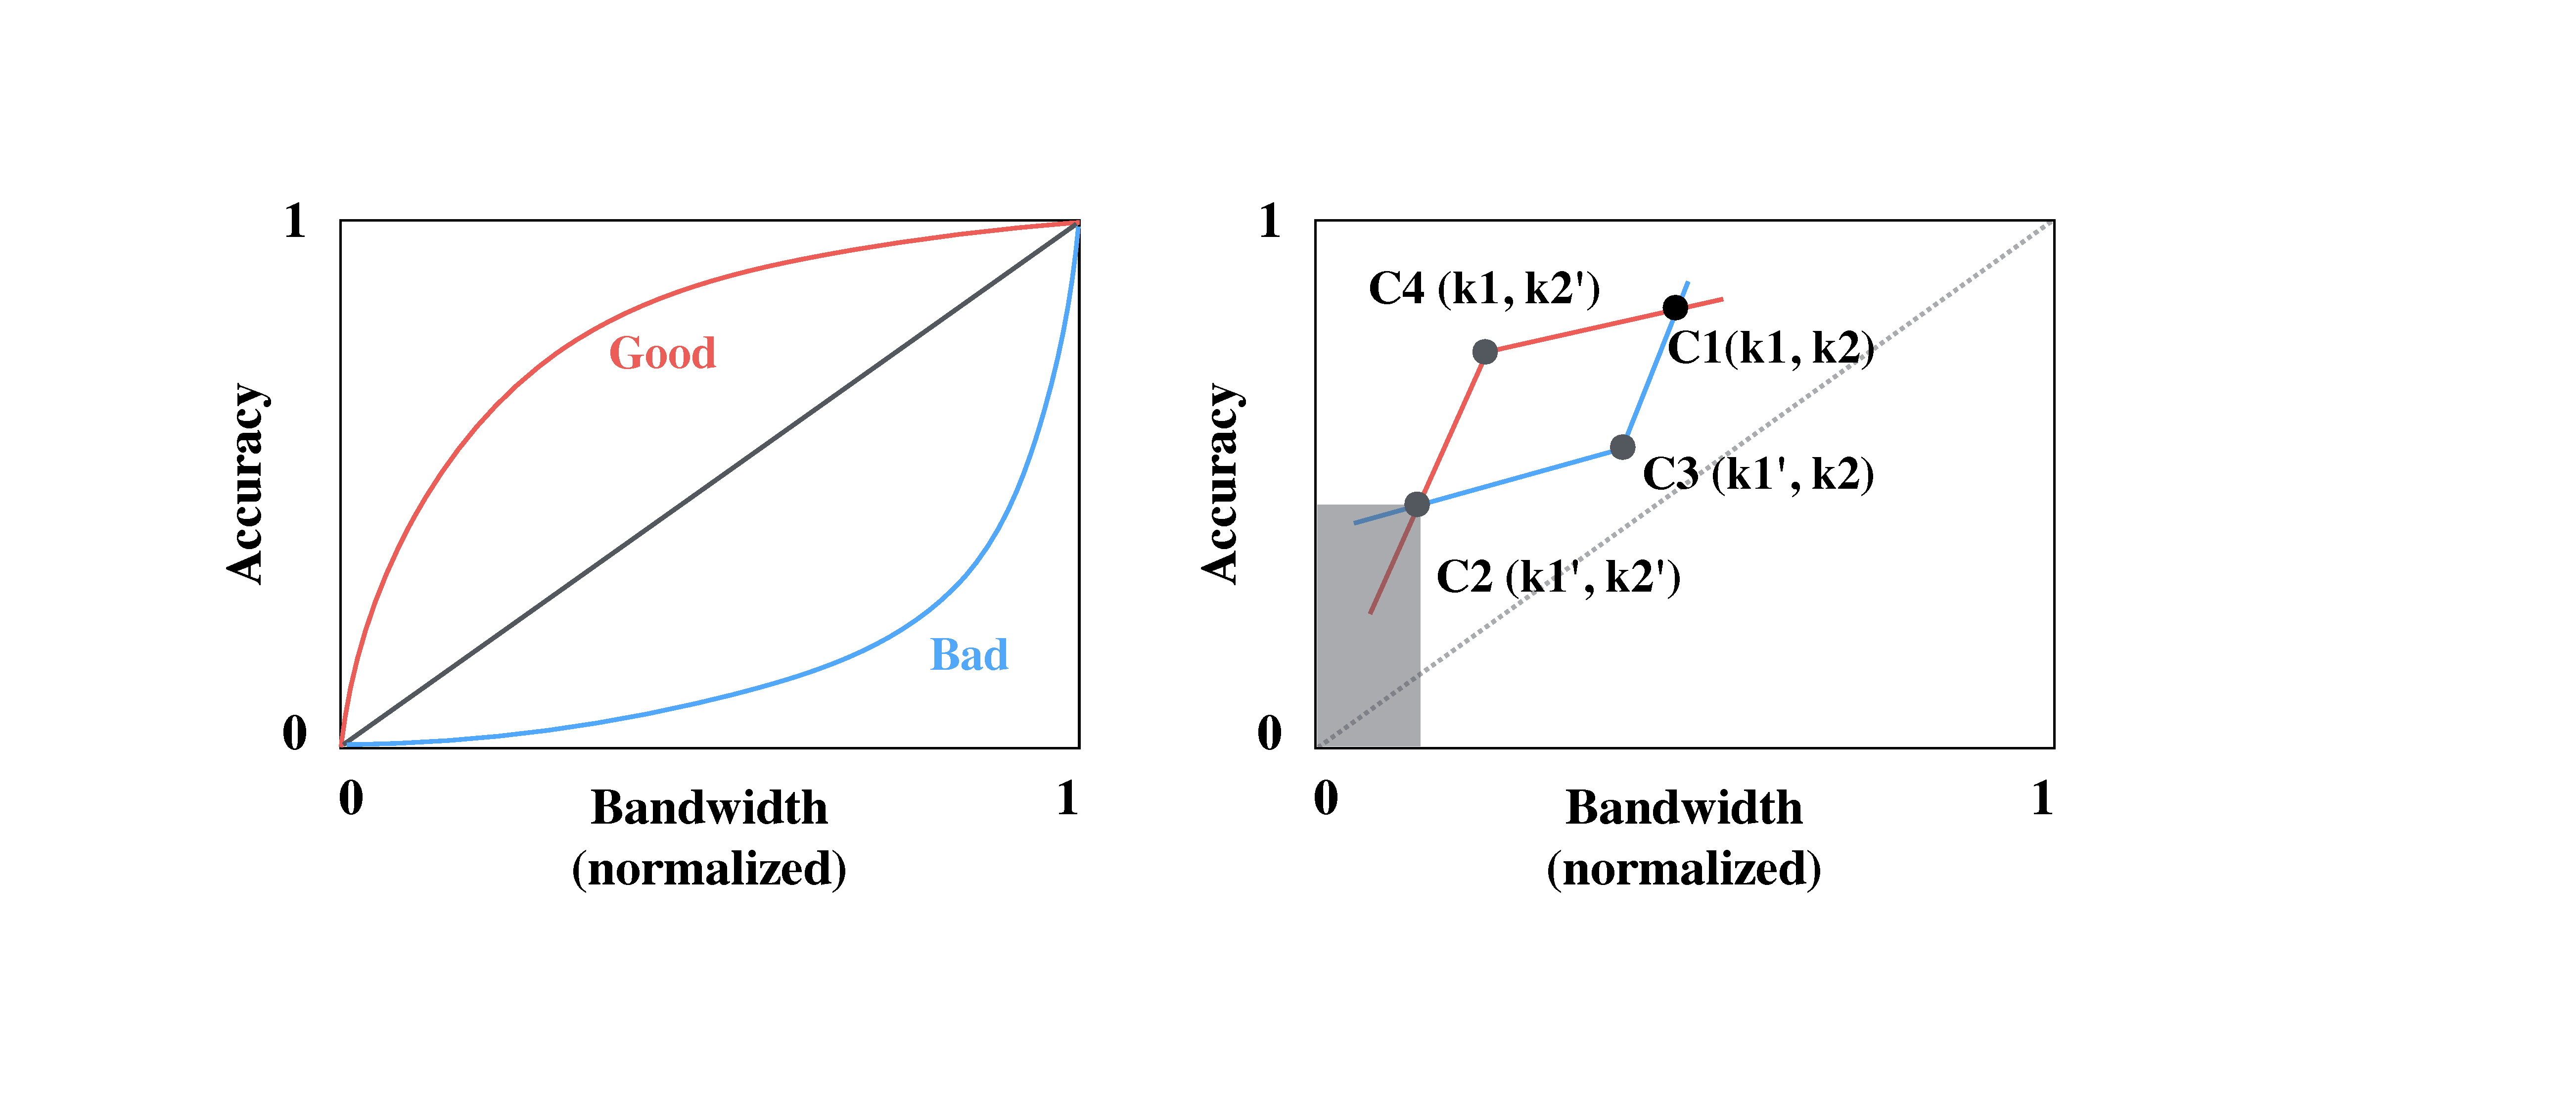
\includegraphics[width=\columnwidth]{figures/degrade.pdf}
  \caption{Illustration on the behavior of different degradation operations.}
  \label{fig:bat}
\end{figure}

When only one knob is involved, we can represent its impact using
bandwidth-accuracy curve (\autoref{fig:bat} left). The point on the curve has a
coordinate $(B(c), A(c))$ for configuration $c$. The straight line from (0, 0)
to (1, 1) splits the space into two parts. Along this line, the amount of
bandwidth saving leads to an equal amount of accuracy drop (when both quantities
are normalized to 1). If a degradation's profile lies above this line, it
indicates an effective degradation that should be employed as it offers little
accuracy drop with more bandwidth savings. For degradation operations below the
straight line, data information loss is more severe than the savings when the
degradation is in effect. One way to capture the relative power of different
degradation strategy is to use the area under the curve (AUC). With this setup,
the Pareto-optimal strategy can be define as the curve that has a maximal AUC.
We will show some concrete profile curves in~\autoref{sec:evaluation}.

While $B(c)$ and $A(c)$ are usually monotonic along individual dimension $k_i$,
when multiple degradations combined, each curve may have a distinct shape. The
right side of \autoref{fig:bat} illustrates this complex
relationship. \todo{write more}.

Although the complexity of degradation operations prohibits further
optimizations to reduce the profiling time, there are several techniques in
practice that can make the problem tractable: (i) Exploring these configurations
is an offline task; there is no direct dependencies among configurations,
resulting in an embarrassingly parallel task. Executed in a cluster, it scales
out perfectly with provided compute resources. (ii) When the degradation level
increases or when multiple degradation operations are in effect, the amount of
data to be analyzed becomes smaller; also the computational complexity for each
data item can also be dramatically reduced. (iii) Developers can specify a lower
bound on the accuracy and the profiling can stop exploring worse configurations.
Once there is a known configuration that is worse than the configured threshold,
configurations with a larger level of degradation do not need to be profiled
(such as the gray area in \autoref{fig:bat}).

\section{Runtime Adaptation}
\label{sec:adaptation}

\begin{figure}
  \centering
  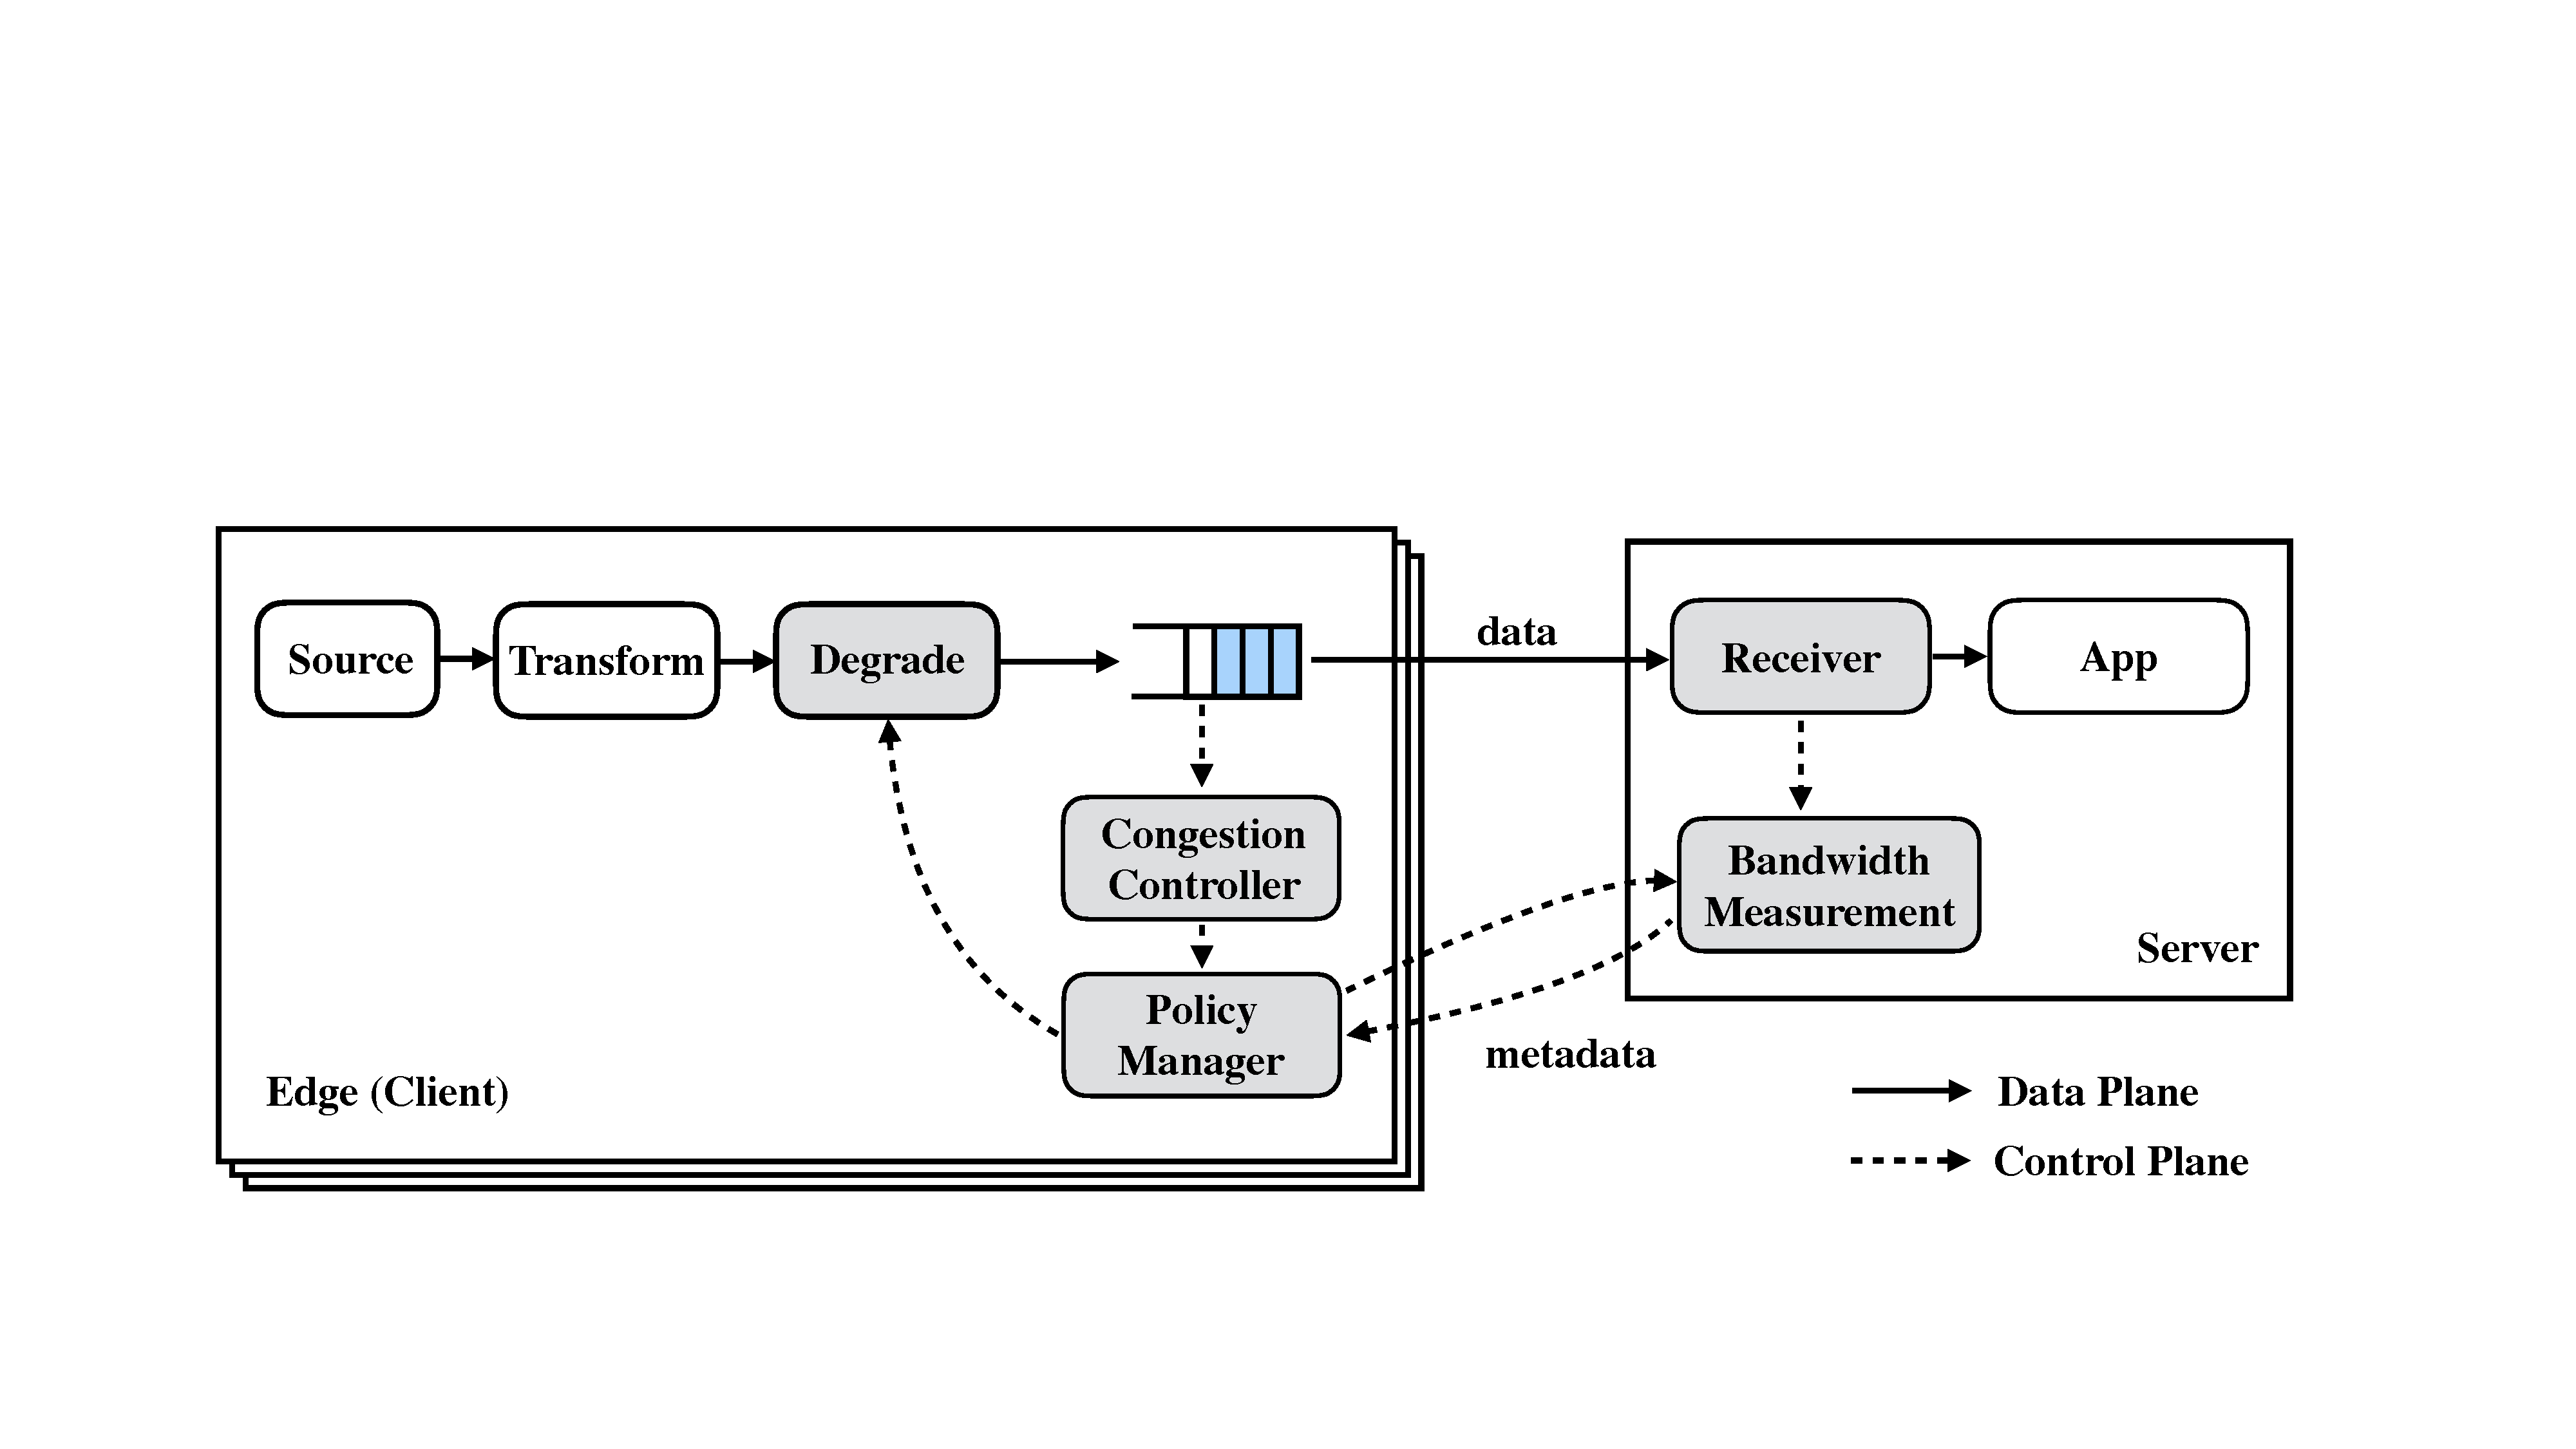
\includegraphics[width=\linewidth]{figures/runtime.pdf}
  \caption{Runtime adaptation system architecture. \sysname{}'s provided
    components are grey: they form the control plane to compensate the
    application's data plane.}
  \label{fig:runtime}
\end{figure}

At runtime, \sysname{} provides the necessary modules for an automatic
adaptation. \autoref{fig:runtime} shows the architecture of \sysname{}
runtime. Applications are split into a client half and server half and they
interact with each other under the control of \sysname{}. We detail the
functionality of each module as follows:

\para{Object-level queue:} The queue bridges data generation from the
application and handles its mismatch with the network resource. When the network
capacity is sufficient, the queue will at most have one object in the process of
being transmitted. Network congestion creates backlogged data that are placed
inside this queue. The queue is being monitored by the congestion controller to
detect congestion.

\para{Congestion controller:} Whenever a new object enqueues, the congestion
controller keeps track of the number of objects as well as the queued data size
(in bytes). Using the queue length alone is not enough to determine congestion
status because some degradation operations (such as \texttt{maybe\_skip}) will
change the rate of data generation. Using the data size alone also doesn't work
because degradation operations such as \texttt{maybe\_downsamples} will alter
the data size of individual object. In \sysname{} design, we've adopted an
approach with an adaptive size for congestion signaling: developers configure an
tolerance on the communication delay and the threshold is derived based on the
current configuration.

\para{Bandwidth Measurement:} The receiver delivers the received data from the
network to the application. In the meantime, it measures the effective
throughput between each client-server pair as an indication of current available
bandwidth~\cite{iperf}. To avoid spikes in the bandwidth measurement,
exponential smoothing is employed. The receiver performs bandwidth estimation
every second; but it does not send the information back to each client. In this
way, we avoid unnecessary communication overhead. When the client detects
congestion, it will query the latency with a remote procedure call (RPC).

\para{Policy Manager:} Upon receiving signals from congestion controller, it
performs an RPC request to the server for current bandwidth measurement. Using
the measurement, together with the learned profile from the last stage, it
determines the degradation level. In the case of congestion, the policy manager
will take a conservative approach: using a constant modifier that's smaller than
one to adjust the available bandwidth. On the other hand, when the congestion is
resolved, the policy manager gradually reduce the degradation level. This is
similar to the additive increase phase in TCP congestion control.

\para{Degrade:} To achieve the actual degradation operation, it is in fact quite
simple. Operators based on the \texttt{maybe} APIs support a \texttt{set}
function that would change the internals of the operator. The control plane will
invoke the \texttt{set} function with appropriate parameter to adjust the
degradation level.

%%% Local Variables:
%%% mode: latex
%%% TeX-master: "thesis"
%%% End:

\section{Implementation}
\label{sec:implementation}

While our proposed API is general and not language specific, we have implemented
\sysname{} prototype in Rust (\textasciitilde 4000 lines of code). \sysname{} is
open source on GitHub.\footnote{URL elided for anonymity.}  Applications use
\sysname{} as a library and configure the execution mode---profiling, runtime as
client, or runtime as server---with command line arguments.

% \begin{figure}
%   \centering
%   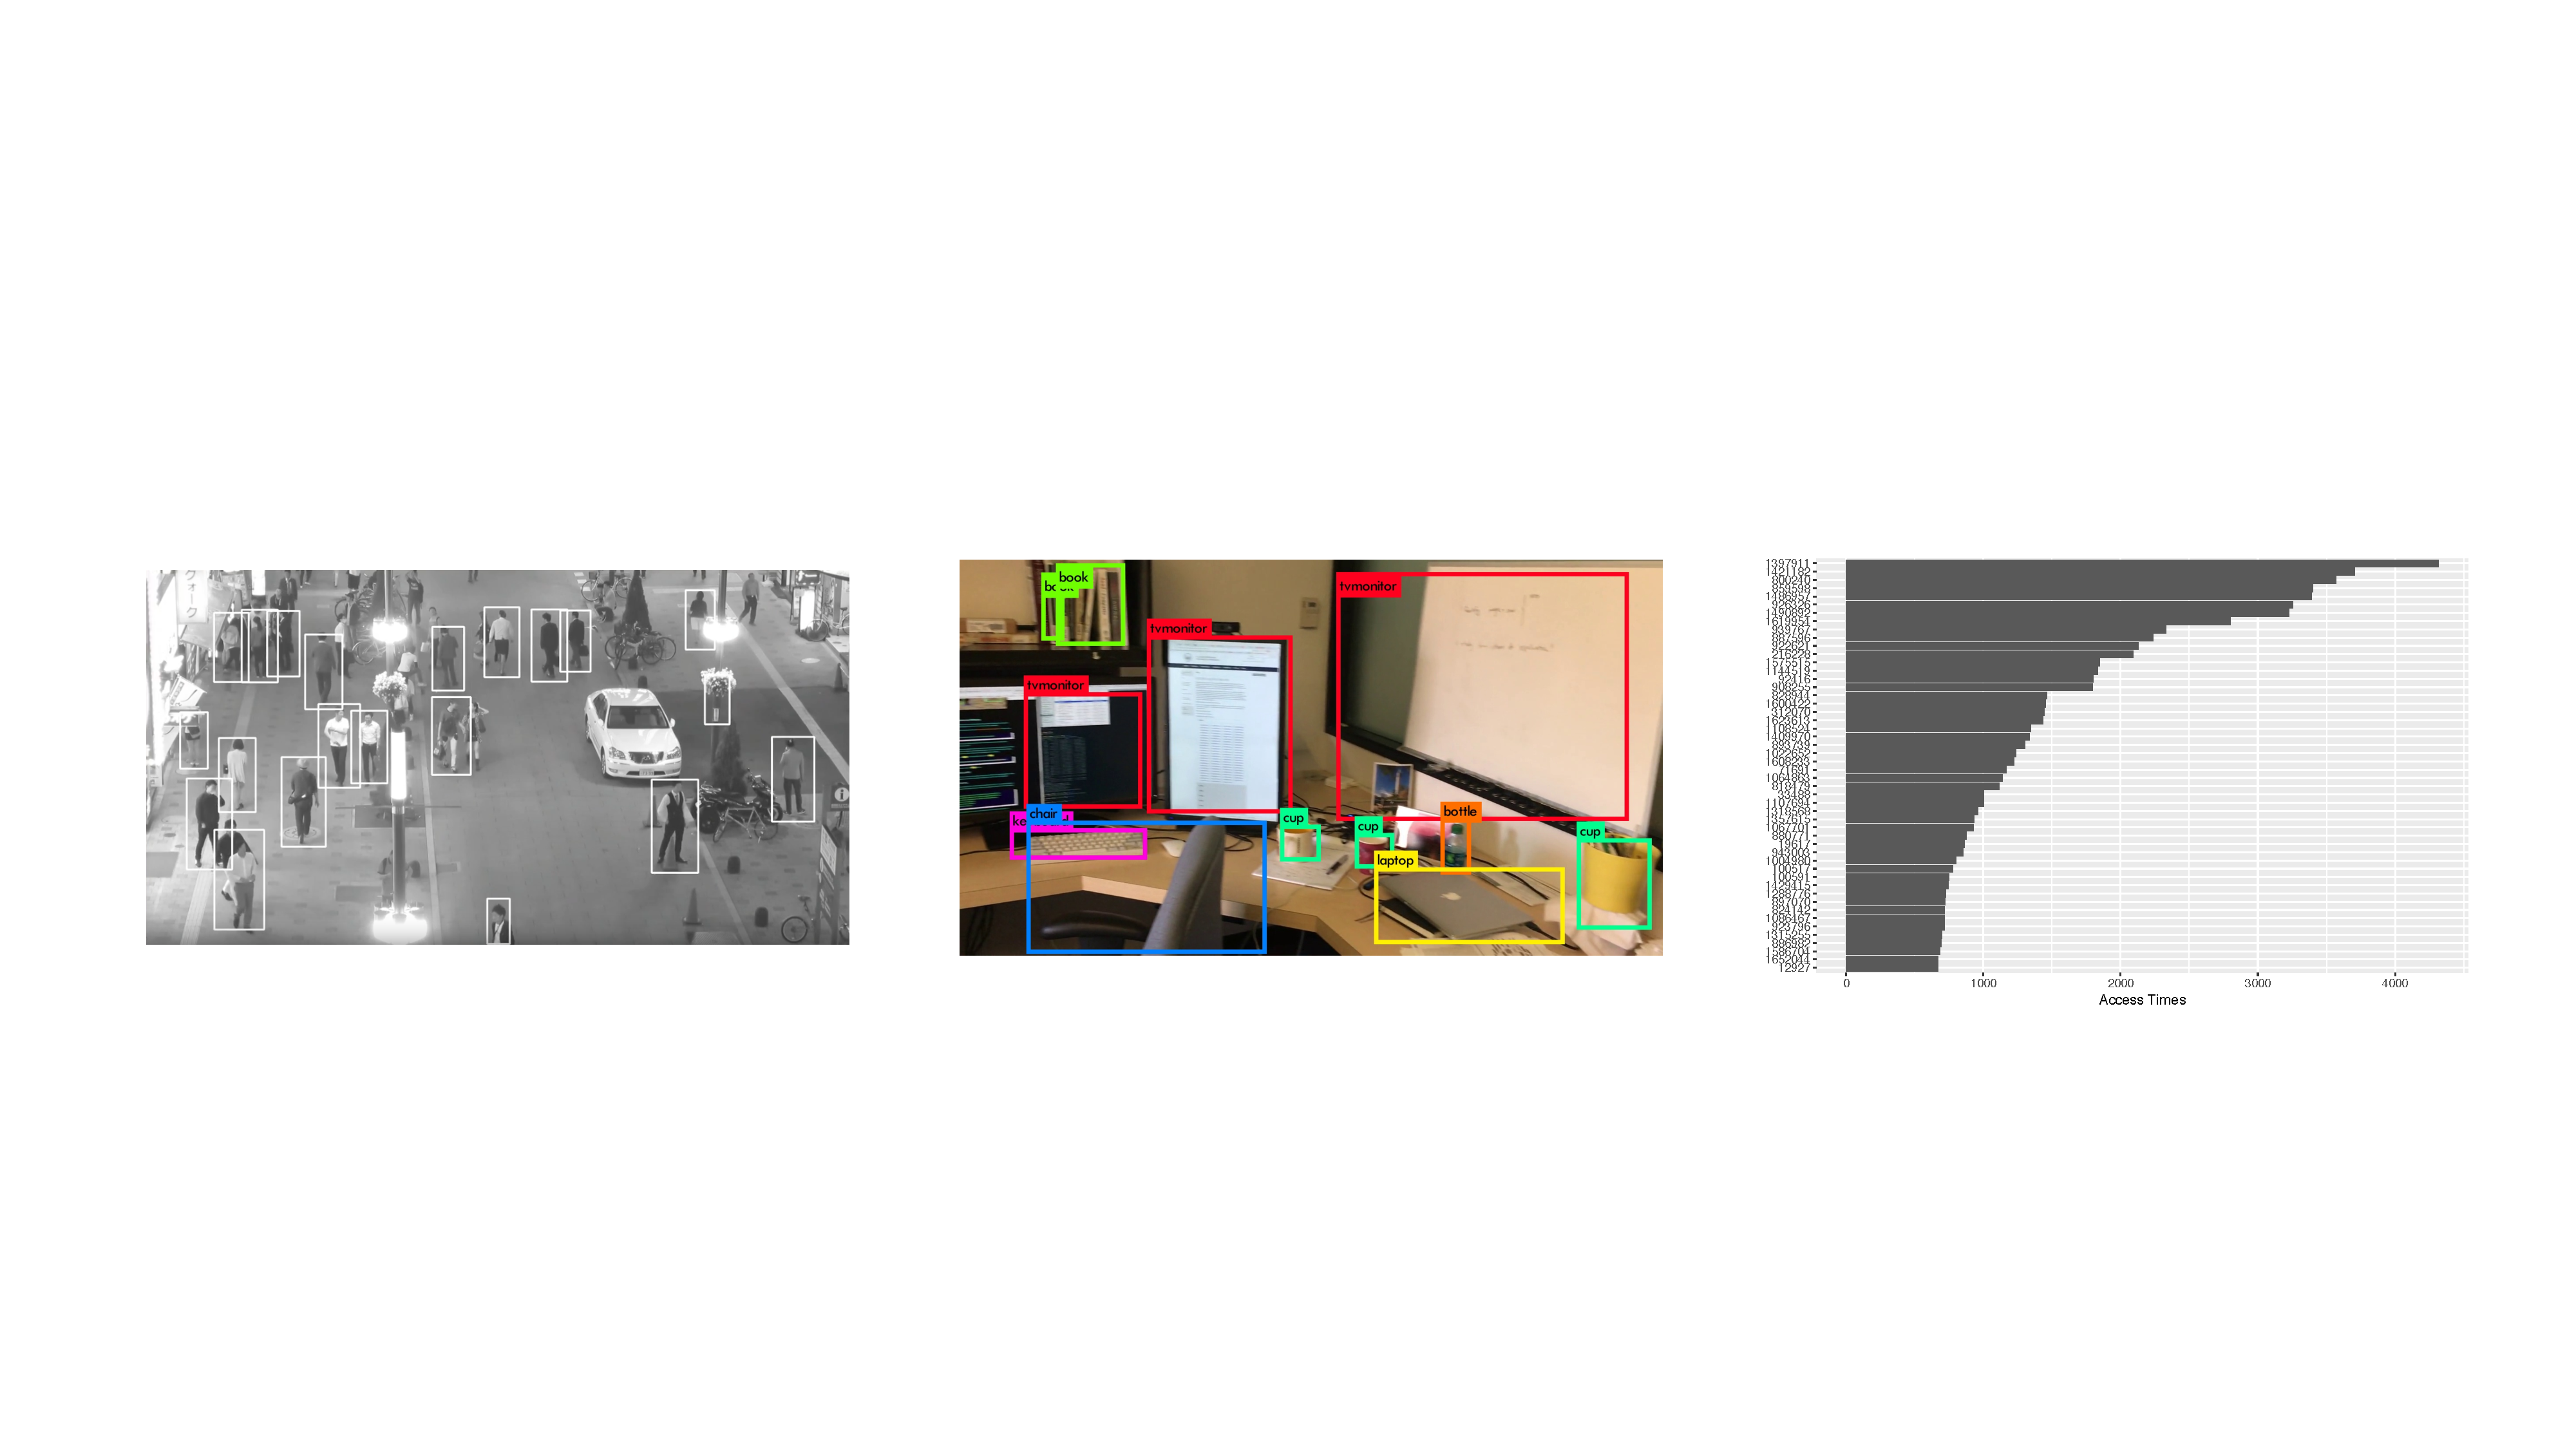
\includegraphics[width=\columnwidth]{figures/apps.pdf}
%   \caption{Three \sysname{} applications: augmented reality, pedestrian
%     detection, and distributed Top-K.}
%   \label{fig:three-apps}
% \end{figure}

\begin{table}
  \footnotesize
  \centering
  \begin{tabular}{c c c c}
    \toprule
    Application & Knobs & Accuracy & Dataset \\
    \midrule
    \specialcell{Augmented\\Reality}
                & \specialcell{resolution \\ frame rate \\ quantization }
                & F1 score~\cite{van1979information}
                & \specialcell{iPhone video clips\\training: office (24
    s)\\testing: home (246 s)} \\
    \midrule
    \specialcell{Pedestrian\\Detection}
                & \specialcell{resolution \\ frame rate \\ quantization }
                & F1 score
                & \specialcell{MOT16~\cite{milan2016mot16}\\training: MOT16-04\\testing: MOT16-03} \\
    \midrule
    \specialcell{Log Analysis\\(Top-K, K=50)}
                & \specialcell{head (N) \\ threshold (T) }
                & \specialcell{Kendall's $\tau$~\cite{abdi2007kendall}}
                & \specialcell{\href{https://www.sec.gov}{SEC.gov} logs~\cite{edgarlog} \\ training: 4 days \\
    testing: 16 days} \\
    \bottomrule
  \end{tabular}
  \vspace{0.5em}
  \caption{Application details.}
  \label{tab:apps}
  \vspace{-1em}
\end{table}

Using \sysname{}, we have built three applications: augmented reality (AR) that
recognizes nearby objects on mobile phones, pedestrian detection (PD) for
surveillance cameras, and a distributed log analysis to extract the Top-K mostly
accessed files (TK). \autoref{tab:apps} summarizes the application-specific
parts: knobs, accuracy functions, and datasets.

\para{Augmented Reality.} We target at augmented reality applications running on
mobile phones that recognize nearby objects by offloading the heavy computation
elsewhere, e.g.\,the cloud.

Our implementation uses OpenCV~\cite{opencvlibrary} for image-related operations
and YOLO~\cite{darknet13, redmon2016yolo9000}, a GPU-enabled pre-trained neural
network, for object recognition. Videos are encoded with
H.264~\cite{richardson2011h}. Our implementation uses GStreamer~\cite{gstreamer}
with \texttt{x264enc} plugin (\texttt{zerolatency} and constant quality). The
quantization factor affecting encoding quality becomes a knob in addition to
image resolutions and frame rates.

Object recognition returns a list of bounding boxes with the object type. Each
bounding box is a rectangle with normalized coordinates on the image. We compare
the detection against the reference result from raw data, and declare it success
if the intersection over union (IOU) is greater than
50\%~\cite{everingham2010pascal} and the object type matches. We use F1
score~\cite{Rijsbergen:1979:IR:539927} as the accuracy function. In terms of
dataset, we collected our own video clips: the training data is a 24-second long
video of an office environment; the test data is a 246-second long video of a
home environment.

\para{Pedestrian Detection.} This application analyzes streams of videos from
installed CCTV cameras and detects pedestrians inside. We use a similar setup
(OpenCV and GStreamer) as our augmented reality application except for the
analytical function. To detect pedestrians, we use GPU-accelerated histogram of
oriented gradients (HOG)~\cite{dalal2005histograms} with the default linear SVM
classifier from OpenCV. Because we do not recognize individual pedestrians, a
successful detection in this case only requires matching the bounding box. Our
evaluation uses MOT16 dataset~\cite{milan2016mot16} for both profiling and
runtime.

\begin{figure}
  \centering
  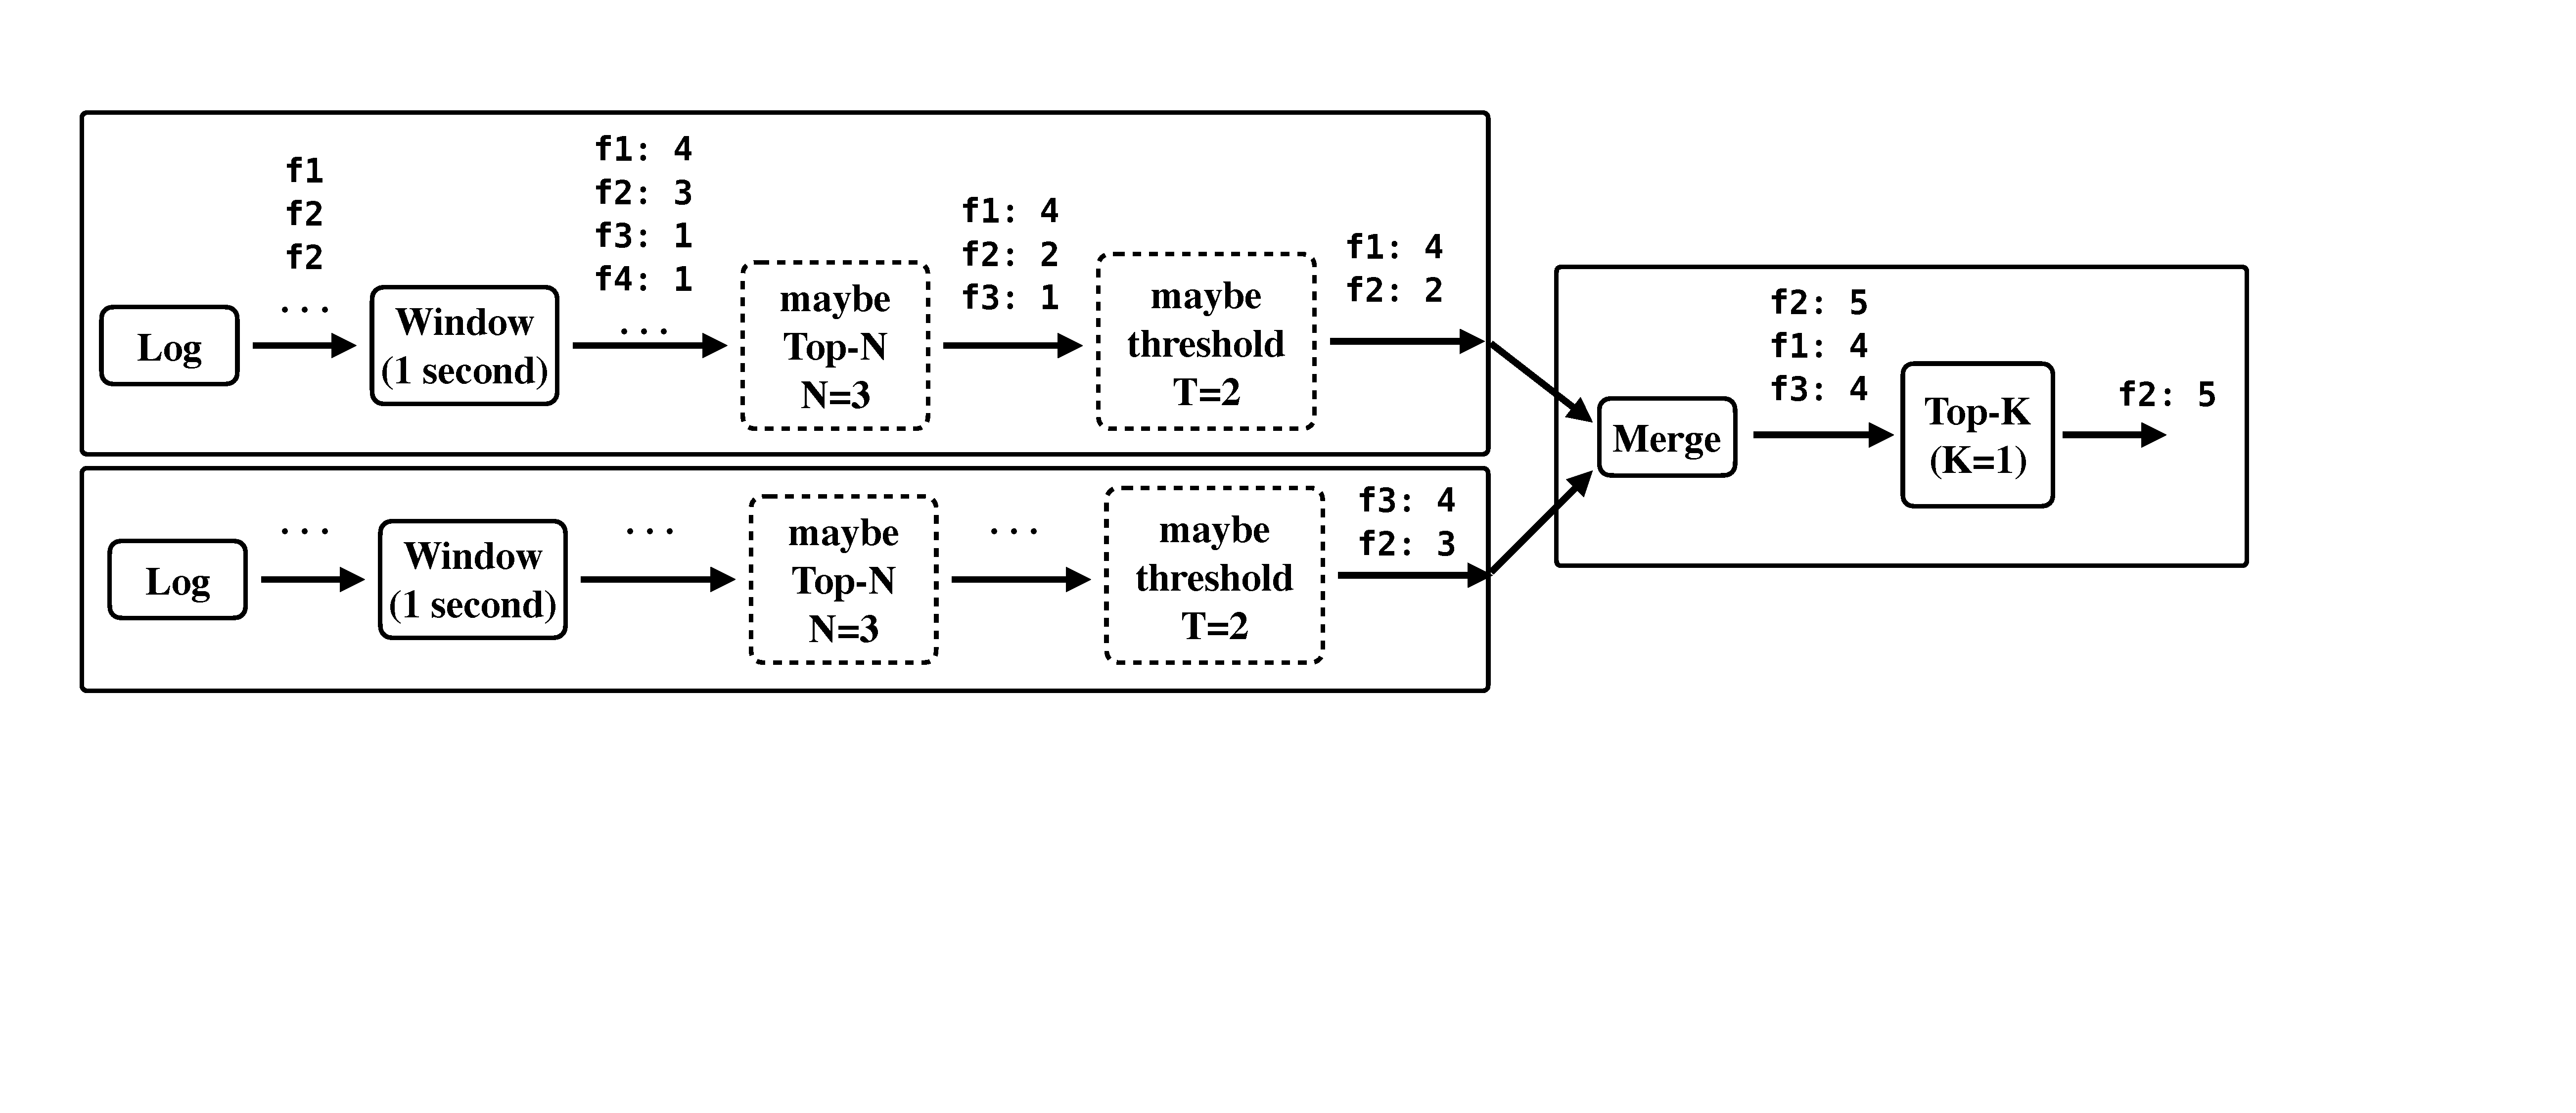
\includegraphics[width=\columnwidth]{figures/topk.pdf}
  \caption{A distributed Top-K application with two degradation operations:
    \texttt{head} and \texttt{threshold}. In this example, \texttt{f2}, which is
    not in Top-1 for either client, becomes the global Top-1 after the merge. It
    would have been purged if the clients use threshold T=3, demonstrating
    degradation that reduces data sizes affects fidelity.}
  \label{fig:topk}
  \vspace{-0.5em}
\end{figure}

\para{Distributed Top-K.} This application aggregates machine logs from
geo-distributed servers to find out the Top-K most accessed files, similar to
many Top-K queries~\cite{babcock2003distributed}.

\autoref{fig:topk} illustrates our processing pipeline with two degradation
operations. First each source node summarizes the log using \texttt{Window}
operator to reduce the data size, a pre-processing step. As many real-world
access patterns follow a long tail distribution, there can be a
large-but-irrelevant tail that contributes little to the final Top-K. Each
source node then filters the tail: (1) head(\texttt{N}) takes the top \texttt{N}
entries; (2) threshold(\texttt{T}) filters small entries whose count is smaller
than \texttt{T}. These two operations affect the final result and the exact
impact depends on data distribution. We implement these two operators by using
\sysname{}'s \maybe{} abstraction.

To measure the accuracy, we need to compare the correlation between two ranked
list. Kendall's~$\tau$~\cite{abdi2007kendall} is a correlation measure of the
concordance between two ranked list. The output ranges from \(-1\) to 1,
representing no agreement to complete agreement. To integrate with \sysname{},
we convert Kendall's~$\tau$ to [0, 1] with a linear transformation. For our
evaluation, we set K as 50 and use Apache log files that record and store user
access statistics for the \href{https://www.sec.gov}{SEC.gov} website. The logs
are split into four groups, simulating four geo-distributed nodes monitoring web
accesses. To match the load of popular web servers, we compress one hour's logs
into one second.

%%% Local Variables:
%%% mode: latex
%%% TeX-master: "../awstream"
%%% End:

%% LocalWords: runtime dataset quantization geo
\chapter{Thesis Plan}
\label{cha:thesis-plan}

This thesis aims to make the following statement: a system-level design that
empowers adaptation in an automatic way will enable the resilient execution of
diverse streaming applications.

The current research results presented in this manuscript, i.e.\,the proposal,
demonstrate how such a design achieves a balance between delay and application
utility in the presence of network resource variation.

The complete thesis will extend the current work to a more holistic framework.
Specifically, I plan to work on the following two directions (see
\autoref{tab:plan} for the concrete timeline):

\para{Multitask resource allocation:} Many streaming applications will co-exist
and share the infrastructure. When uncoordinated, they will compete for
resources such as the network bandwidth. While the adaptation strategy may be
optimal for each application, taking them collectively, the system may not be at
an optimal state. In this direction, I will study the multitask resource
allocation and how it can adapt each streaming applications for an overall
maximal utility.

\para{Adaptation to computing resources:} In addition to network resources, the
computing resources also have a large variation across the heterogeneous
platforms. The available platforms range from embedded devices to powerful
rack-level machines. Also, the availability of the platforms is not always
guaranteed: nodes join and leave; the connectivity may be completely cut off. In
this direction, I will study how to adapt applications to different
configurations of the computing resources.

\vspace{1.5em}
\begin{table}[h]
  \normalsize
  \centering
  \begin{tabular}{r l}
    \toprule
    \textbf{Time} & \textbf{Research Topic} \\
    \midrule
    Spring 2017 & Resource allocation among multiple streaming applications \\
    Summer 2017 & Preliminary study on adaptation to computing resources \\
    Fall 2017 & Combine network and compute resources for a holistic control plane \\
    Spring 2018 &  Finish the thesis \\
    \bottomrule
  \end{tabular}
  \caption{Thesis Timeline}
  \label{tab:plan}
\end{table}

%%% Local Variables:
%%% mode: latex
%%% TeX-master: "thesis"
%%% End:


\printbibliography

\end{document}

%%% Local Variables:
%%% mode: latex
%%% TeX-master: t
%%% End:
